%chap2
\chapter{Analyse et conception}


\thispagestyle{empty}

\newpage

%================header and footer============


\sethead{}{}{Analyse des besoins}\headrule



%==============Début

 \section{Analyse}
 
\subsection{Modèle du cycle de vie}

\subsection{Raffinement des cas d'utilisations}

   
   \begin{enumerate}[label=(\alph*)]
   \item {Diagramme détaillé de cas d'utilisation \textless  Demander l'ouverture d'un dossier AVA \textgreater}
   
    \begin{figure}[!h]
\begin{center}

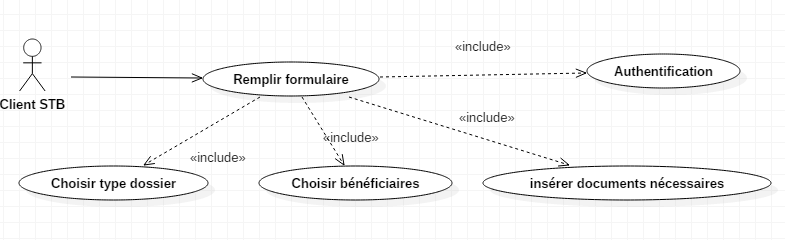
\includegraphics[width=10cm]{./conception/use_case_ouverture}

\caption{Diagramme détaillé de cas d'utilisation demande d'ouverture d'un dossier AVA.}
\end{center}
\end{figure}
 
  Le client du STB peut demander, en ligne, la création d'un dossier AVA en remplissant un formulaire.
Ce dernier contient des informations concernant son type d'activité, compte dans la banque STB, etc.
Le Client peut ajouter des bénéficiaires et choisir leurs états (désactivé, à activer, actif, non actif).
À la fin du formulaire, il doit insérer des fichiers PDF qui varient selon le type du dossier choisi.
 

   
    \item{Diagramme détaillé de cas d'utilisation \textless Annulation de voyage \textgreater}
    
     \item{Diagramme détaillé de cas d'utilisation \textless Rétrocession \textgreater}
     
     \item{Diagramme détaillé de cas d'utilisation \textless Ajouter un Bénéficiaire \textgreater}
     
      \item{Diagramme détaillé de cas d'utilisation \textless Désactiver un Bénéficiaire \textgreater}
    \end{enumerate}    
 


 \section{Conception}
 
 \subsection{Diagrammes d'activités}
 
 \subsubsection{Diagrammes de séquence \textless Demande d'ouverture d'un dossier AVA \textgreater}

\begin{figure}[!h]
 \begin{center}
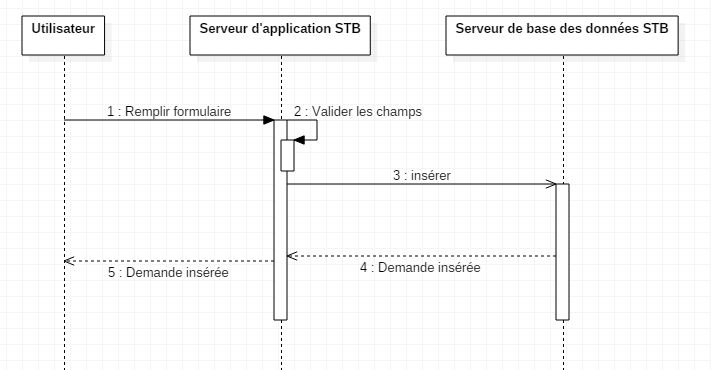
\includegraphics{./conception/sequence_ouverture}

%légende de l'image
\caption{Diagramme de séquence\textless ouverture dossier AVA\textgreater}
\end{center}
\end{figure}

%description textuelle
\begin{itemize}
\item  Description textuelle \\
Titre : Demande d'ouverture d'un dossier AVA.\\
Acteur principal : client du STB.\\
Résumé : Le client du STB doit pouvoir demander en ligne la création d'un dossier AVA.\\

Scénario nominal\\
\begin{enumerate}
\item Le client choisit l'interface d'ouverture d'un dossier AVA.
\item Il remplit un formulaire d'ouverture.
\item Il valide le formulaire.
\item Le système valide les champs saisis.
\item Le système trouve que le client n'a pas un dossier AVA ouvert.
\item Notification de la création de la demande.
\end{enumerate}
\end{itemize}

  \subsubsection{Diagrammes d'activité \textless Rétrocession \textgreater}
  
  \subsection{Diagrammes de séquences}
  
  \subsubsection{Diagramme de séquence \textless s'authentifier \textgreater}
  
  \subsubsection{Diagramme de séquence \textless Ajouter bénéficiaire \textgreater}
  
  \subsection{Diagramme des classes global}
  
  %inclusion d'une mage dans le document
\begin{figure}[!h]


%remplacer "width" par "height" pour régler la hauteur

\begin{center}
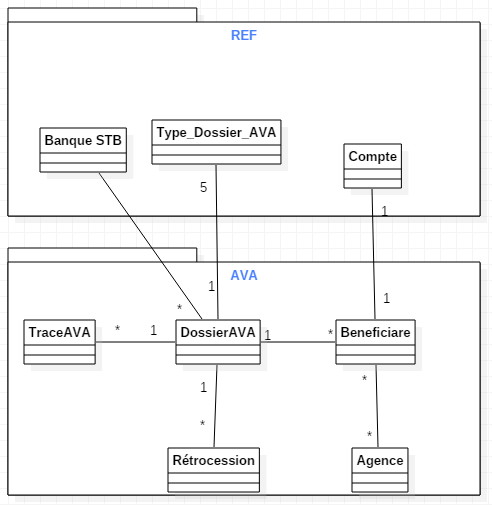
\includegraphics{./conception/diagramme_classes}

%légende de l'image
\caption{Diagramme des classes global}
\end{center}
\end{figure}
  
  
  
  
 

 
 
 

 